\chapter{绪论}
\section{研究背景}
随着计算机视觉(Computer Vision)
和自然语言处理(Natural Language Processing)技术的迅猛发展,
跨模态智能理解成为人工智能研究的重要方向之一。
其中,视觉问答(Visual Question Answering, VQA)\cite{goyal2017making}任务因其广泛的应用前景和挑战性,
受到了学术界和工业界的广泛关注。

视觉问答是一种多模态任务,它要求计算机能够基于给定的图像内容,
理解并回答关于该图像的自然语言问题。例如,给定一幅包含动物的图片,
系统需要能够回答“这只动物是什么颜色?”或“图片中有几只猫?”等问题。
这一任务的核心在于多模态信息的深度融合,即如何在视觉特征和语言信息之间建立有效的联系。

VQA 技术的研究涉及多个领域,
包括计算机视觉中的目标检测(Object Detection)、
图像分类(Image Classification)、图像语义分割(Semantic Segmentation),
以及自然语言处理中的文本理解(Text Understanding)、语义解析(Semantic Parsing)等。
近年来,深度学习的快速发展极大地推动了 VQA 技术的进步,
尤其是基于卷积神经网络(Convolutional Neural Networks, CNNs)
和循环神经网络(Recurrent Neural Networks, RNNs)的方法,使得计算机能够更好地理解和生成答案。

视觉问答在多个实际应用场景中具有重要价值。
例如,在辅助盲人阅读图像信息、自主机器人理解环境、医疗影像分析、教育和娱乐等方面,
VQA 技术都可以提供智能化的交互方式,提高系统的可用性和便利性。
然而,由于数据的不确定性、语言表达的多样性、以及多模态信息融合的复杂性,
VQA 仍然面临诸多挑战,例如开放域问题的泛化能力、推理能力的提升、以及对长尾问题的有效应对等。

为了解决这些挑战,研究人员提出了多种 VQA 模型架构,
包括基于注意力机制(Attention Mechanism)\cite{Bahdanau2015Attention}、
图神经网络(Graph Neural Networks, GNNs)、
预训练视觉-语言模型(Pretrained Vision-Language Models)等方法,以提高 VQA 系统的理解能力和回答质量。

大语言模型(Large Language Model)

回答集编程(Answer Set Programming,ASP)是一种声明式编程范式,可用于解决复杂的
人工智能问题。ASP起源于对逻辑编程、非单调推理和知识表示的研究。ASP因其具有表达
性声明性的语言和以Clingo为代表的一些高效实现而流行起来。ASP已经在学术界和
工业界得到广泛应用,并被证明在人工智能的几个知识密集型应用中能够有效解决问题,
如调度、产品配置、机器人、劳动力管理和决策支持等。
ASP能够以简洁和直观的方式来表示知识,允许用户相对容易地去表示复杂问题,
而且ASP具有分单调推理的特性,允许不完整信息的表示和默认推理。
另外,ASP对知识的表达能力,使得其支持集成各种类型的知识,包括规则、约束和偏好,有助于灵活解决问题。

\section{相关研究现状}
视觉问答(Visual Question Answering, VQA)作为一种多模态任务,近年来受到了广泛关注。
研究者们提出了多种方法来提升 VQA 模型的性能,包括基于深度学习的端到端模型、注意力机制、图神经网络
以及预训练的视觉-语言模型等。
\subsection{传统VQA方法}
早期的 VQA 研究主要依赖于特定的特征提取和简单的模型架构。
例如,Antol 等人(2015)提出了最早的大规模 VQA 数据集 VQA v1,
并基于长短时记忆网络(LSTM)与卷积神经网络(CNN)构建了一个简单的 VQA 基线模型\cite{Antol2015VQA}。
然而,这类方法在处理复杂推理任务时存在一定局限。
\subsection{深度学习驱动的VQA}
近年来,随着深度学习的快速发展,基于神经网络的方法成为 VQA 研究的主流。
Anderson 等人(2018)提出了基于注意力机制的 Bottom-Up and Top-Down(BUTD)模型,
该方法在 VQA 任务上取得了显著提升\cite{Anderson2018BUTD}。
此外,Tan 和 Bansal(2019)探索了视觉和语言的联合预训练方法,提出了 LXMERT,
一个专门为多模态任务设计的 Transformer 模型\cite{Tan2019LXMERT}。
\subsection{基于多模态预训练的VQA}
近年来,预训练模型在 VQA 任务中取得了突破性进展。
例如,Radford 等人(2021)提出了 CLIP(Contrastive Language-Image Pretraining),
通过大规模图像-文本数据进行对比学习,使得模型在零样本 VQA 任务上表现优异\cite{Radford2021CLIP}。Li 等人(2020)提出了 UNITER,
一种统一的视觉-语言表示学习框架,能够在多个 VQA 数据集上实现最先进的性能\cite{Li2020UNITER}。
\subsection{可解释性与推理能力增强的VQA}
虽然深度学习驱动的 VQA 模型在性能上取得了显著进步,但它们的可解释性和推理能力仍然是一个重要的研究问题。
Gokhale 等人(2020)提出了一种基于因果推理的 VQA 方法,以减少数据偏差的影响\cite{Gokhale2020CausalVQA}。
此外,研究者们探索了基于知识图谱(Knowledge Graph)和符号推理的方法,以增强 VQA 的推理能力。
例如,Hudson 和 Manning(2019)提出的 MAC 网络引入了可解释的记忆组件,以模拟逐步推理\cite{Hudson2019MAC}。

\section{研究目标与内容}

\section{研究方法与技术路线}

\section{论文结构}
本文共分为六个章节,各章节的主要内容具体如下:

第一章为绪论,总体介绍本文的研究背景及意义、相关研究现状与不足、研究目标
与研究内容、研究方法与技术路线及本文的结构安排。

第二章

第三章

第四章

第五章

第六章中对本文工作加以总结,并展望未来工作。

\nomenclature{PF}{powerful fingers}
如图\ref{lxfbook}所示。

\begin{figure}
    \centering
    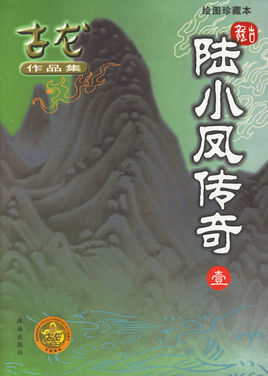
\includegraphics[width=.6\textwidth]{lxfbook.jpg}
    \caption{陆小凤传奇\label{lxfbook}}
\end{figure}
\nomenclature{KF}{kung fu}